\documentclass[11pt,a4paper]{article}

\usepackage[margin=1in]{geometry}
\usepackage{graphicx}
\usepackage{booktabs}
\usepackage{amsmath}
\usepackage{amssymb}
\usepackage{array}
\usepackage{caption}
\usepackage{verbatim}
\usepackage[hidelinks]{hyperref}

% siunitx is not installed in this minimal TinyTeX (tlmgr is cross-release
% locked, TeX Live 2025 vs 2026 remote), so define the few unit macros we use.
\newcommand{\celsius}{\ensuremath{^\circ}C}
\newcommand{\SI}[2]{#1\,#2}

% listings is likewise not installable here, so emulate \lstinputlisting with
% the core verbatim package: print the file name as a heading, then its body.
\newcommand{\lstset}[1]{}
\newcommand{\lstinputlisting}[2][]{%
  \par\medskip\noindent\textbf{\ttfamily\footnotesize #2}\par\nopagebreak
  \vspace{2pt}\hrule\vspace{2pt}%
  {\scriptsize\verbatiminput{#2}}\vspace{1pt}\hrule\medskip}

\graphicspath{{../figures/}}

\captionsetup{font=small,labelfont=bf}
\setlength{\parskip}{4pt}
\setlength{\parindent}{0pt}

\title{\vspace{-1.2cm}\textbf{Fuzzy Logic Control for an Intelligent Assistive Care Environment:\\
Design, Genetic Optimisation, and a Comparison of Evolutionary Optimisers\\ on CEC'2005 Benchmark Functions}}

\author{Rahul Karn (250163) \and Rashant Nayaju (250117)}

\date{Module: STW7085CEM Advanced Machine Learning \\
Softwarica College / Coventry University \\
\today}

\begin{document}
\maketitle

\begin{abstract}
\noindent
This report presents Task 2 of the Advanced Machine Learning module: an evolutionary and fuzzy
systems study built and simulated in MATLAB R2026a using the Fuzzy Logic Toolbox and the Global
Optimization Toolbox. We first design a Mamdani fuzzy logic controller (FLC) that regulates the
thermal comfort of one room in an assistive care flat for a resident with reduced mobility. The
controller takes room temperature and resident activity as inputs and produces a single heating or
cooling command. We document every component (membership functions, rule base, inference and
defuzzification) and analyse its behaviour through rule activation, the control surface and a
day-long operational scenario. We then design a real-coded genetic algorithm (GA) that tunes the
controller's membership functions against a target dataset; the GA reduces the mean squared error by
81 percent (from 300.9 to 57.2) and outperforms the built-in \texttt{ga} solver on the same problem.
Finally we compare three optimisers (GA, particle swarm optimisation, and simulated annealing) on two
CEC'2005 functions (F1 Shifted Sphere and F9 Shifted Rastrigin) at dimensions 2 and 10, with 15
independent runs each. The GA is the most robust optimiser on the multimodal Rastrigin function,
particle swarm is strongest on the smooth unimodal Sphere, and simulated annealing is weakest at high
dimension. The hand-coded optimisers are cross-checked against their Global Optimization Toolbox
counterparts and agree closely.
\end{abstract}

%======================================================================
\section{Introduction}
%======================================================================
An intelligent assistive care environment uses sensing and automated control to keep a vulnerable
resident comfortable and safe with little manual intervention. Thermal comfort is one of the most
important services in such an environment: a resident with reduced mobility may not be able to adjust
heating or open a window, and both overheating and excessive cold carry real health risks. A fuzzy
logic controller is well suited to this problem because comfort is naturally expressed in linguistic
terms (the room is ``warm'', the resident is ``active'') and because fuzzy rules encode expert comfort
knowledge directly and transparently.

This report addresses the three parts of the assignment:
\begin{enumerate}
  \item \textbf{Part 1 (design and implementation).} A demonstrable Mamdani FLC for room climate
        control, with full evidence of each component and an analysis of its output behaviour.
  \item \textbf{Part 2 (genetic optimisation).} A genetic algorithm that adjusts the controller's
        membership functions to fit a target dataset, including the encoding, the genetic operators,
        the fitness function and the chromosome length.
  \item \textbf{Part 3 (optimiser comparison).} A comparison of at least two optimisation techniques
        on two CEC'2005 benchmark functions at two dimensions, with statistics over 15 runs and
        convergence graphs.
\end{enumerate}
All work was carried out in MATLAB R2026a. The complete code, figures and result tables accompany this
report and are listed in the appendix.

%======================================================================
\section{Part 1: Design and Implementation of the FLC}
%======================================================================

\subsection{Control scenario and variables}
The controller regulates the climate of a single room (for example the living room) of an assistive
flat. It reads two inputs and drives one actuator:
\begin{itemize}
  \item \texttt{temperature} (\SI{10}{}--\SI{35}{\celsius}): the measured room temperature.
  \item \texttt{activity} (0--10): an activity or occupancy index from motion sensing, where 0 is a
        resting or sleeping resident and 10 is a highly active one.
  \item \texttt{hvac} ($-100$ to $+100$): a single signed actuator command, where negative values call
        for cooling and positive values call for heating. A signed output lets one variable express the
        full heat or cool decision and produces a single, readable control surface.
\end{itemize}
Activity is included because a person's thermally neutral temperature falls as they become more active:
an active resident generates body heat and prefers a cooler room, while a resting resident feels cold
sooner. The controller therefore biases towards cooling as activity rises.

\subsection{Fuzzy sets and membership functions}
Temperature uses five fuzzy sets (Cold, Cool, Comfortable, Warm, Hot), activity uses three (Low, Medium,
High), and the output uses five (StrongCool, Cool, Off, Heat, StrongHeat). Five sets on temperature give
fine resolution around the comfort band where the control action changes most, while three activity sets
are enough to separate resting, normal and active behaviour without an unnecessarily large rule base.
Five output sets let the actuator move in graded steps rather than switching abruptly.

All sets use triangular and trapezoidal membership functions (Figure~\ref{fig:p1mf}). These piecewise
linear shapes are standard for control, are easy to interpret, and are convenient to encode for the
genetic algorithm in Part 2 because each set is defined by only three or four breakpoints. The extreme
sets are trapezoidal (shoulders) so that the controller saturates sensibly beyond the comfort band, and
neighbouring sets overlap at a membership of about 0.5 so that the controller interpolates smoothly
between rules.

\begin{figure}[h]
  \centering
  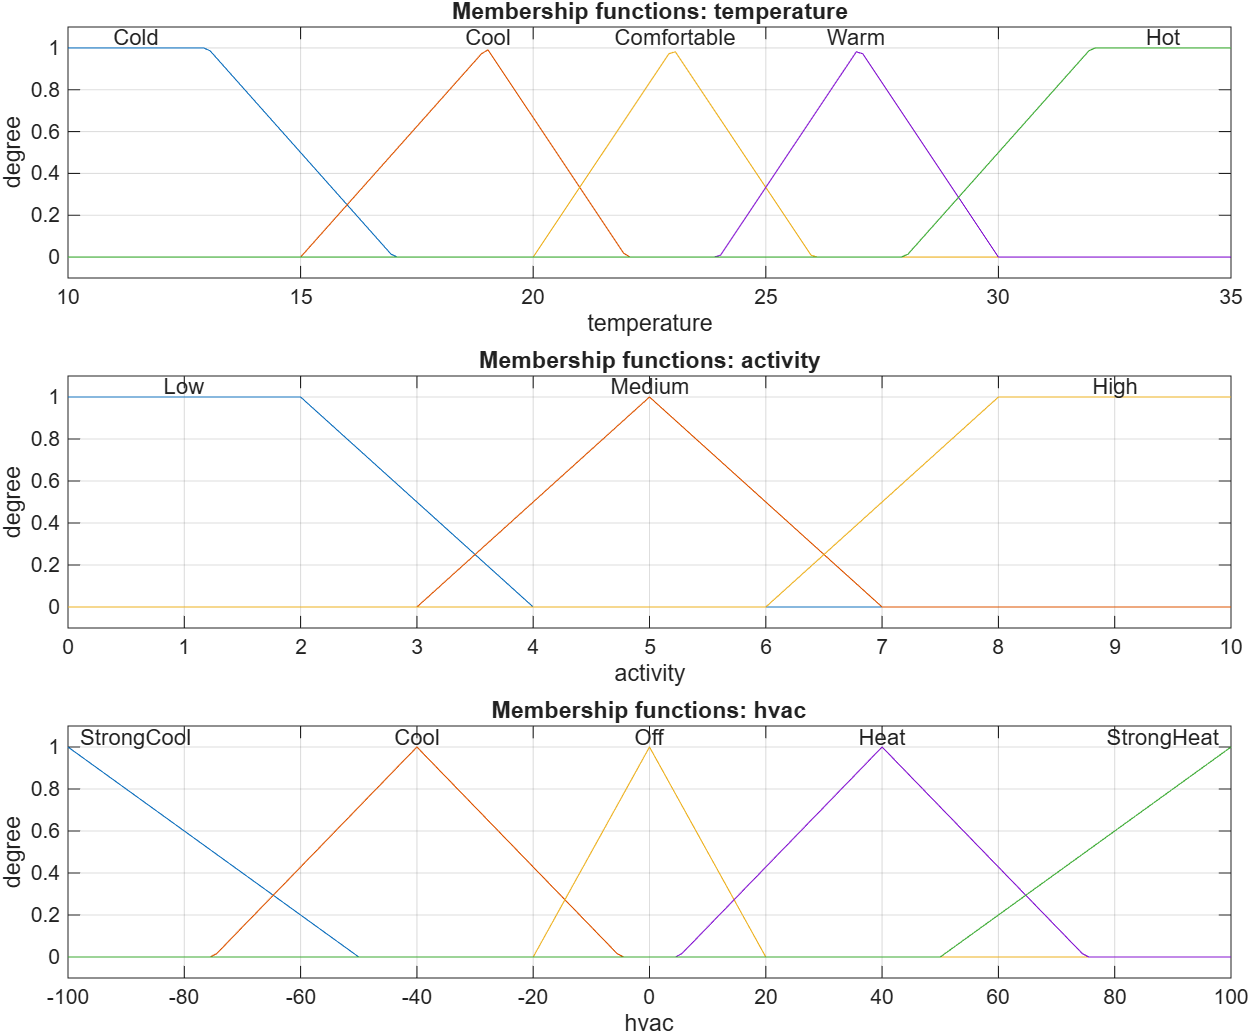
\includegraphics[width=0.92\textwidth]{p1_membership_functions.png}
  \caption{Membership functions for the two inputs and the output. Temperature is partitioned into five
  overlapping sets, activity into three, and the HVAC command into five graded sets from StrongCool to
  StrongHeat. The overlap of about 0.5 between neighbours produces smooth interpolation.}
  \label{fig:p1mf}
\end{figure}

\subsection{Rule base}
The rule base contains $5 \times 3 = 15$ rules, one for each combination of a temperature set and an
activity set, shown in Table~\ref{tab:rules}. The rules encode two comfort principles. First, the HVAC
command opposes the temperature error: a cold room is heated and a hot room is cooled, with the strength
of the action growing as the temperature moves further from comfortable. Second, higher activity shifts
the response towards cooling, so for a fixed temperature an active resident receives less heating or more
cooling than a resting one. For example, a cold room with a resting resident calls for StrongHeat, but the
same cold room with a very active resident calls only for Heat.

\begin{table}[h]
  \centering
  \caption{The 15-rule base. Rows are the temperature set, columns are the activity set, and each cell is
  the resulting HVAC command. The rules are connected with the AND (minimum) operator.}
  \label{tab:rules}
  \begin{tabular}{l ccc}
    \toprule
    \textbf{temperature} $\backslash$ \textbf{activity} & \textbf{Low} & \textbf{Medium} & \textbf{High} \\
    \midrule
    Cold        & StrongHeat & StrongHeat & Heat       \\
    Cool        & Heat       & Heat       & Off        \\
    Comfortable & Off        & Off        & Cool       \\
    Warm        & Cool       & Cool       & StrongCool \\
    Hot         & StrongCool & StrongCool & StrongCool \\
    \bottomrule
  \end{tabular}
\end{table}

\subsection{Inference and defuzzification}
The controller is a Mamdani fuzzy inference system. Mamdani inference is chosen over Sugeno because its
fuzzy consequents make the rule activation and the aggregated output easy to visualise, which directly
supports the evidence required for this part, and because the linguistic outputs (StrongCool, Heat, and
so on) are a natural way to express an actuator command to a non-technical audience. The system uses the
minimum operator for the AND connective and for implication, the maximum operator for aggregation, and
the centroid method for defuzzification. The centroid (centre of area) is the standard Mamdani choice
because it produces a smooth output that takes account of the whole aggregated fuzzy set, which avoids the
abrupt jumps that methods such as mean-of-maximum can cause.

\subsection{Implementation and block diagram}
The system was built in MATLAB with the Fuzzy Logic Toolbox using \texttt{mamfis}, \texttt{addInput},
\texttt{addOutput}, \texttt{addMF} and \texttt{addRule}, and exported as \texttt{room\_flc.fis}
(see \texttt{build\_flc.m} in the appendix). Figure~\ref{fig:p1block} shows the resulting block diagram:
two inputs, one Mamdani inference block and 15 rules driving a single output.

\begin{figure}[h]
  \centering
  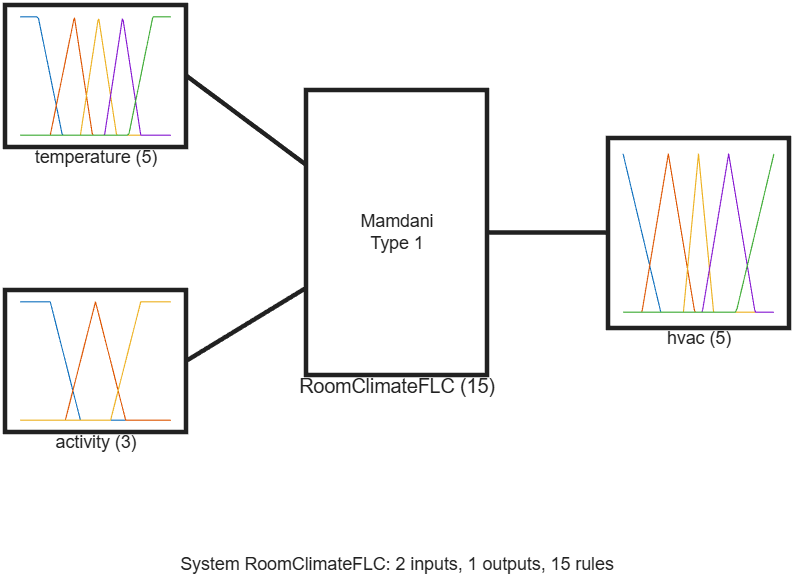
\includegraphics[width=0.7\textwidth]{p1_block_diagram.png}
  \caption{Block diagram of the fuzzy inference system: inputs \texttt{temperature} (5 sets) and
  \texttt{activity} (3 sets), 15 rules, and output \texttt{hvac} (5 sets).}
  \label{fig:p1block}
\end{figure}

\subsection{Output behaviour analysis}
\textbf{Rule activation.} Figure~\ref{fig:p1rule} shows which rules fire for a warm, active situation
(temperature \SI{29}{\celsius}, activity 7). Only the rules whose antecedent sets overlap the inputs are
active: rule 12 (Warm AND High $\rightarrow$ StrongCool) fires with strength 0.33 and rule 15
(Hot AND High $\rightarrow$ StrongCool) with strength 0.25, and the centroid of the aggregated output is
$-79.4$, that is, strong cooling. This is exactly the behaviour expected for a hot room with an active
resident.

\begin{figure}[h]
  \centering
  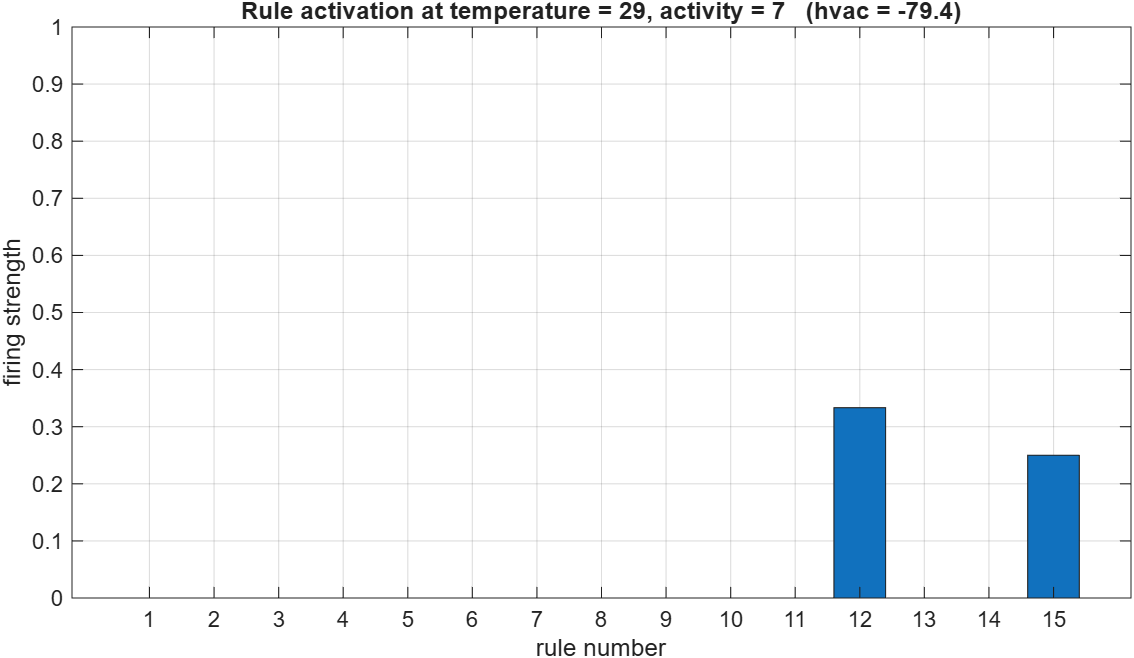
\includegraphics[width=0.8\textwidth]{p1_rule_activation.png}
  \caption{Rule firing strengths at temperature \SI{29}{\celsius}, activity 7. Two rules fire (12 and 15),
  both demanding strong cooling; the defuzzified command is $-79.4$.}
  \label{fig:p1rule}
\end{figure}

\textbf{Control surface.} Figure~\ref{fig:p1surf} is the complete input-output map of the controller. It
is monotonic and smooth: the command rises towards strong heating in the cold, low-activity corner and
falls towards strong cooling in the hot, high-activity corner, with a near-zero band along the comfortable
region. The smoothness confirms that the sets overlap correctly and that there are no gaps or
contradictions in the rule base.

\begin{figure}[h]
  \centering
  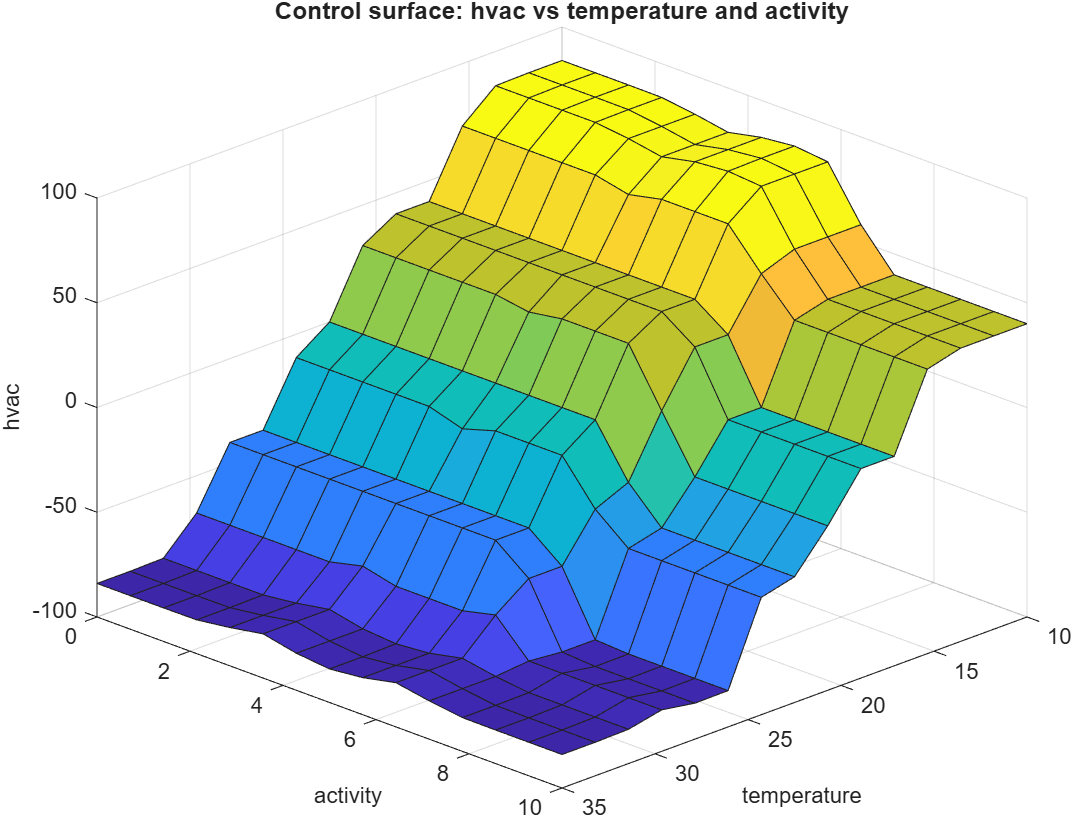
\includegraphics[width=0.72\textwidth]{p1_control_surface.png}
  \caption{Control surface: HVAC command as a function of temperature and activity. The surface is smooth
  and monotonic, heating when cold and cooling when hot, with the cooling bias increasing with activity.}
  \label{fig:p1surf}
\end{figure}

\textbf{Operational scenario.} Figure~\ref{fig:p1scenario} traces the controller across one simulated day
in which the room warms through a busy afternoon and then cools through a quiet evening. The HVAC command
follows correctly: mild heating overnight when the room is cool and the resident is resting, a near-zero
command in the comfortable morning, strong cooling (down to about $-84$) at the warm and active midday
peak, and a return to heating as the evening cools and activity falls. This demonstrates that the
controller meets its intended behaviour over a realistic operating cycle.

\begin{figure}[h]
  \centering
  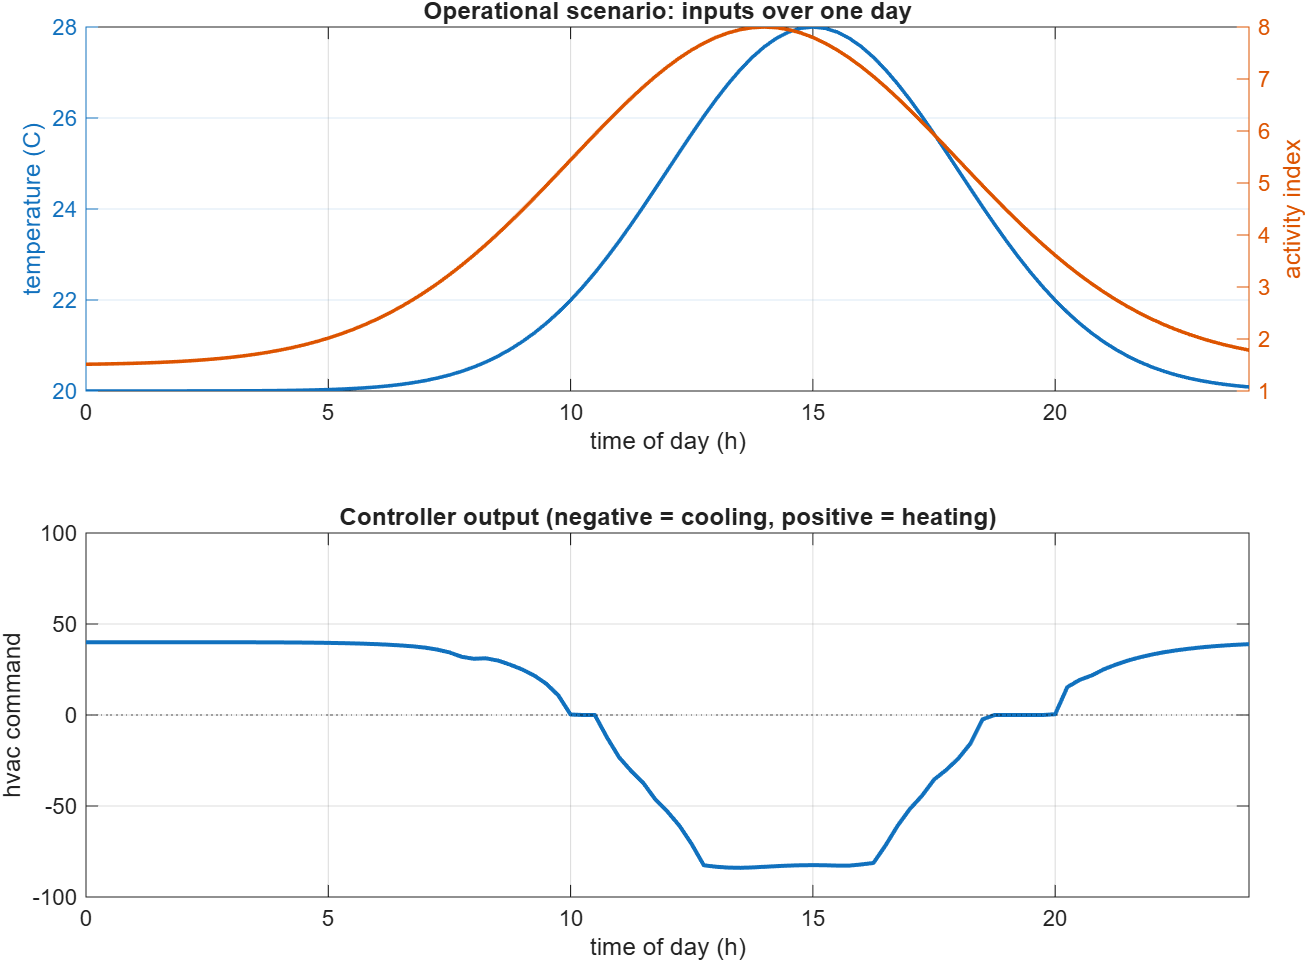
\includegraphics[width=0.9\textwidth]{p1_operational_scenario.png}
  \caption{Operational scenario over 24 hours. Top: the temperature and activity inputs. Bottom: the HVAC
  command, which cools strongly at the warm active midday peak and heats gently during the cool, low
  activity night.}
  \label{fig:p1scenario}
\end{figure}

\clearpage
\subsection{Evidence from the MATLAB Fuzzy Logic Designer}
The figures above are produced programmatically from the exported \texttt{room\_flc.fis}. For completeness,
this section shows the same controller inside the interactive MATLAB Fuzzy Logic Designer, the tool the
brief asks for. Figure~\ref{fig:gui_system} is the system block diagram in the app,
Figure~\ref{fig:gui_mf} shows the membership-function editor for each variable with its parameter table,
Figure~\ref{fig:gui_rules} lists the full 15-rule base in natural language, and
Figure~\ref{fig:gui_infer} is the live Rule Inference view evaluated at the operating point used above
(temperature 29, activity 7), where the defuzzified output is again \(-79.4\).
Figure~\ref{fig:gui_surface} is the interactive control surface in the app.

\begin{figure}[h]
  \centering
  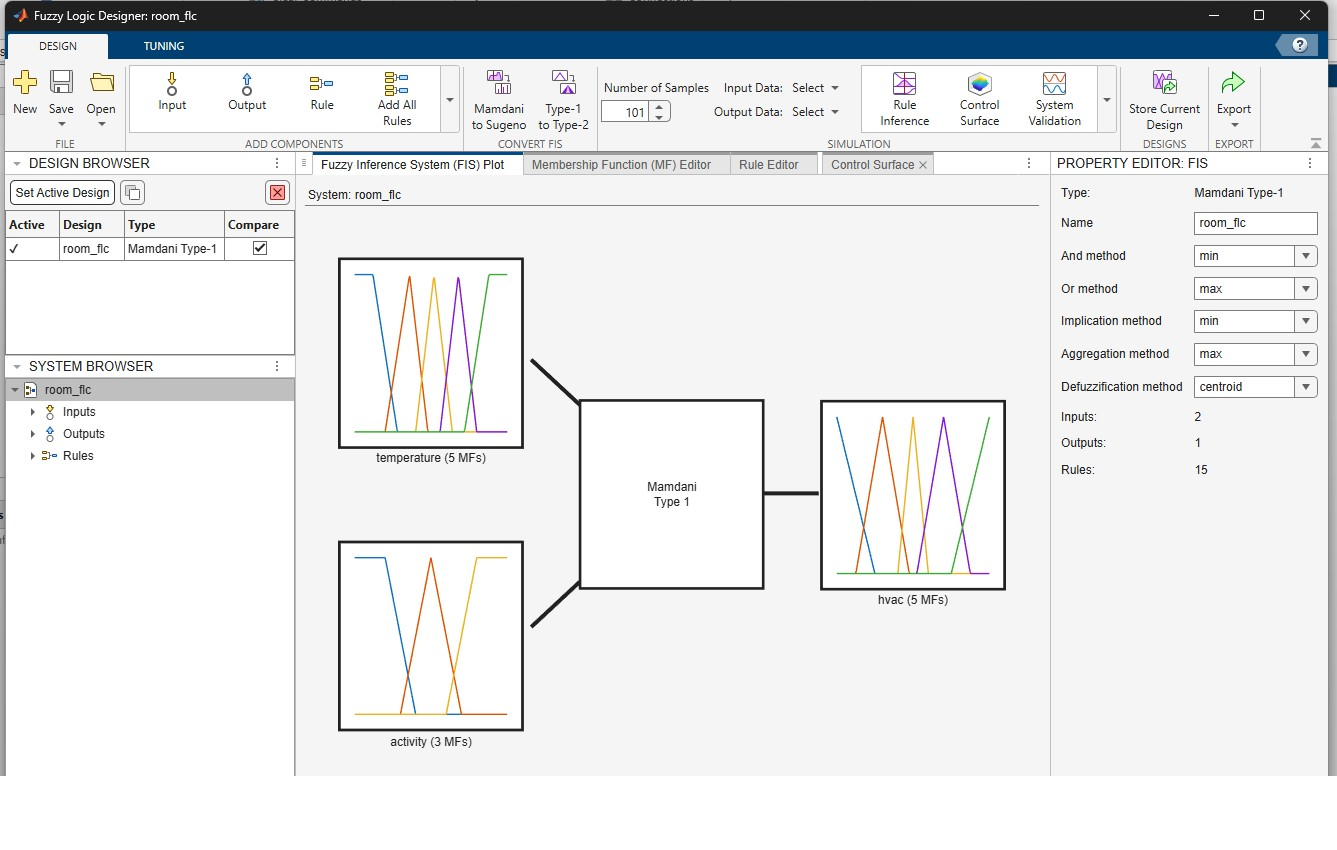
\includegraphics[width=0.92\textwidth]{../realss/gui_02_system.jpg}
  \caption{Fuzzy Logic Designer: the system (FIS) block diagram, with inputs \texttt{temperature} and
  \texttt{activity} feeding the Mamdani inference block and the \texttt{hvac} output.}
  \label{fig:gui_system}
\end{figure}

\begin{figure}[h]
  \centering
  \begin{minipage}{0.82\textwidth}
    \centering
    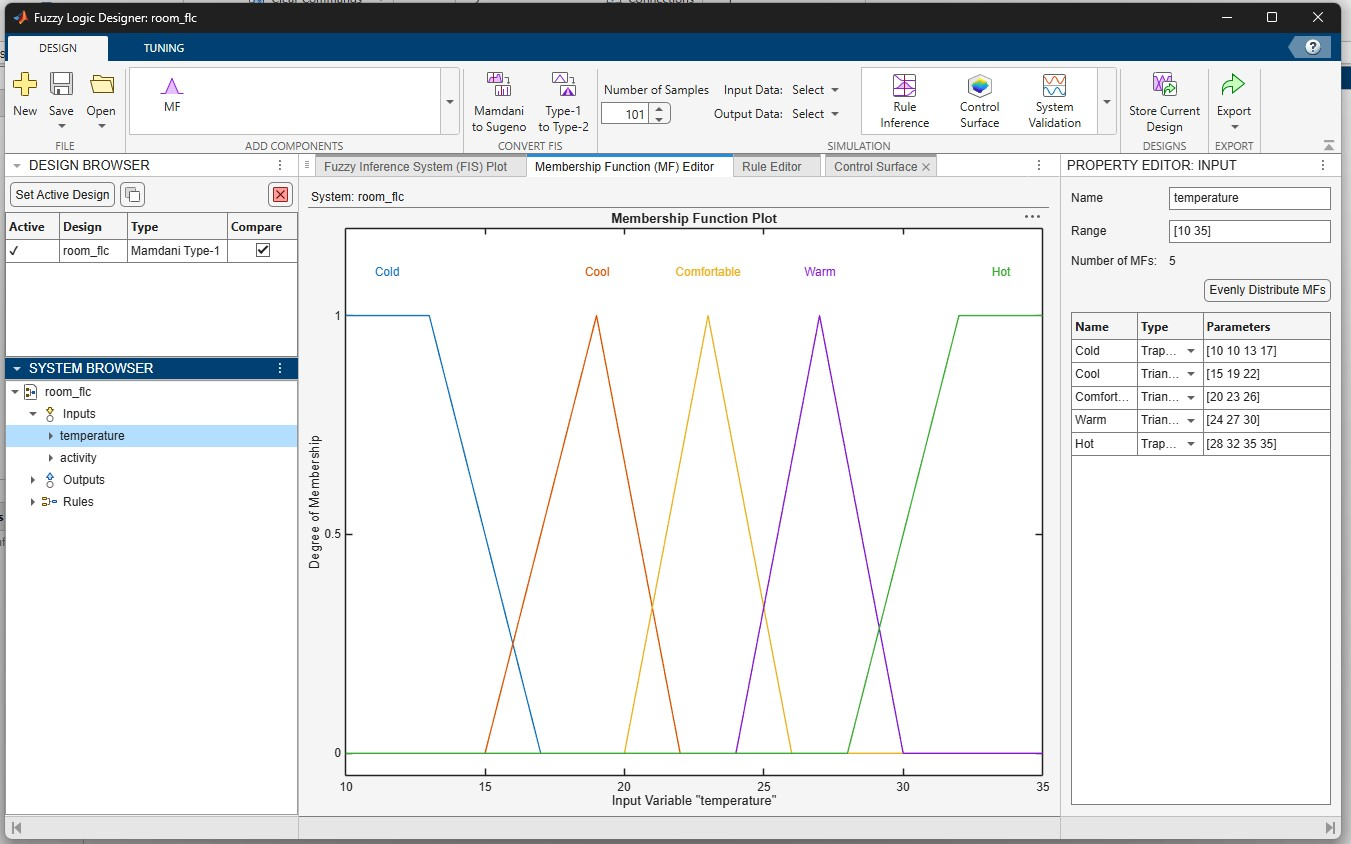
\includegraphics[width=\textwidth]{../realss/gui_03_mf_temperature.jpg}\\[1pt]
    {\small (a) temperature}
  \end{minipage}\\[4pt]
  \begin{minipage}{0.82\textwidth}
    \centering
    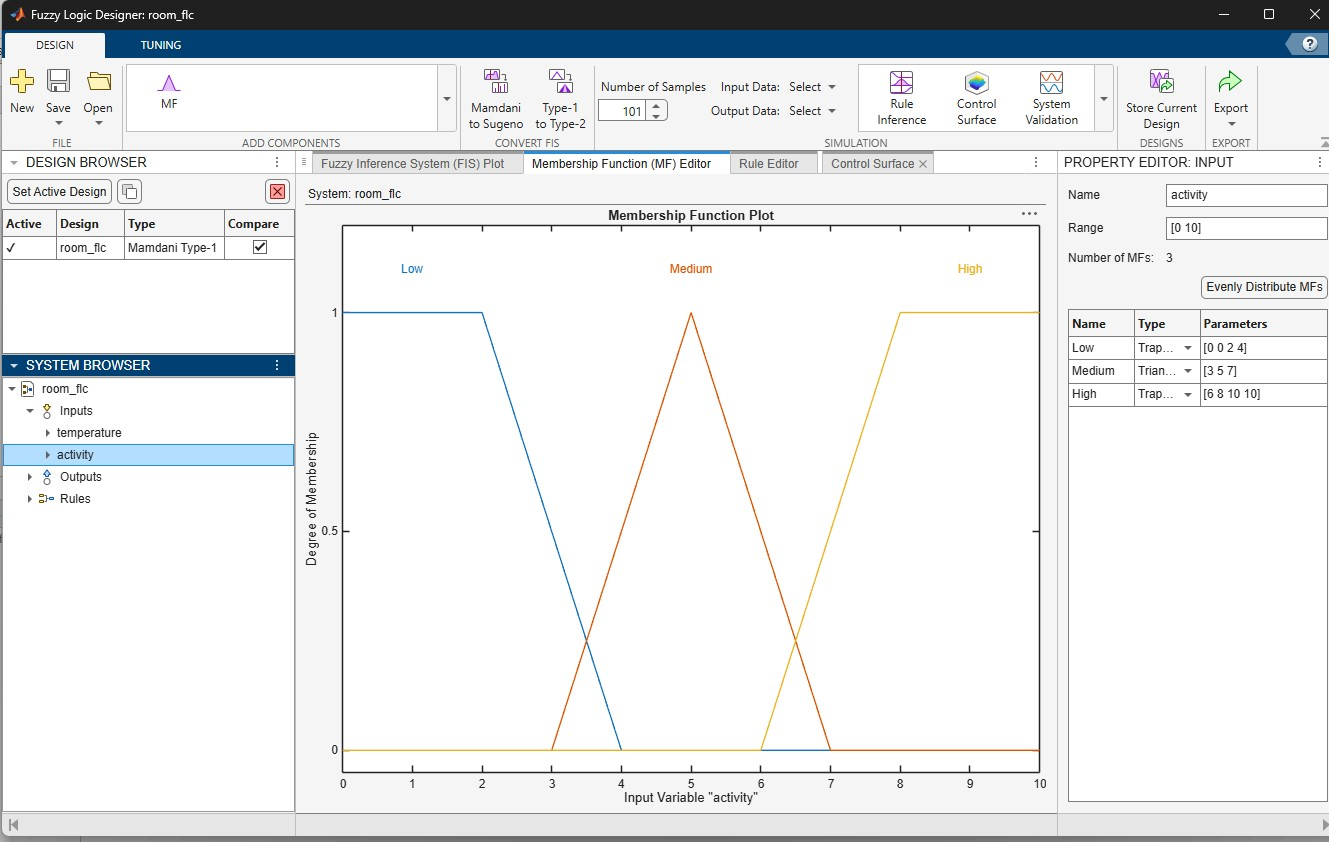
\includegraphics[width=\textwidth]{../realss/gui_04_mf_activity.jpg}\\[1pt]
    {\small (b) activity}
  \end{minipage}\\[4pt]
  \begin{minipage}{0.82\textwidth}
    \centering
    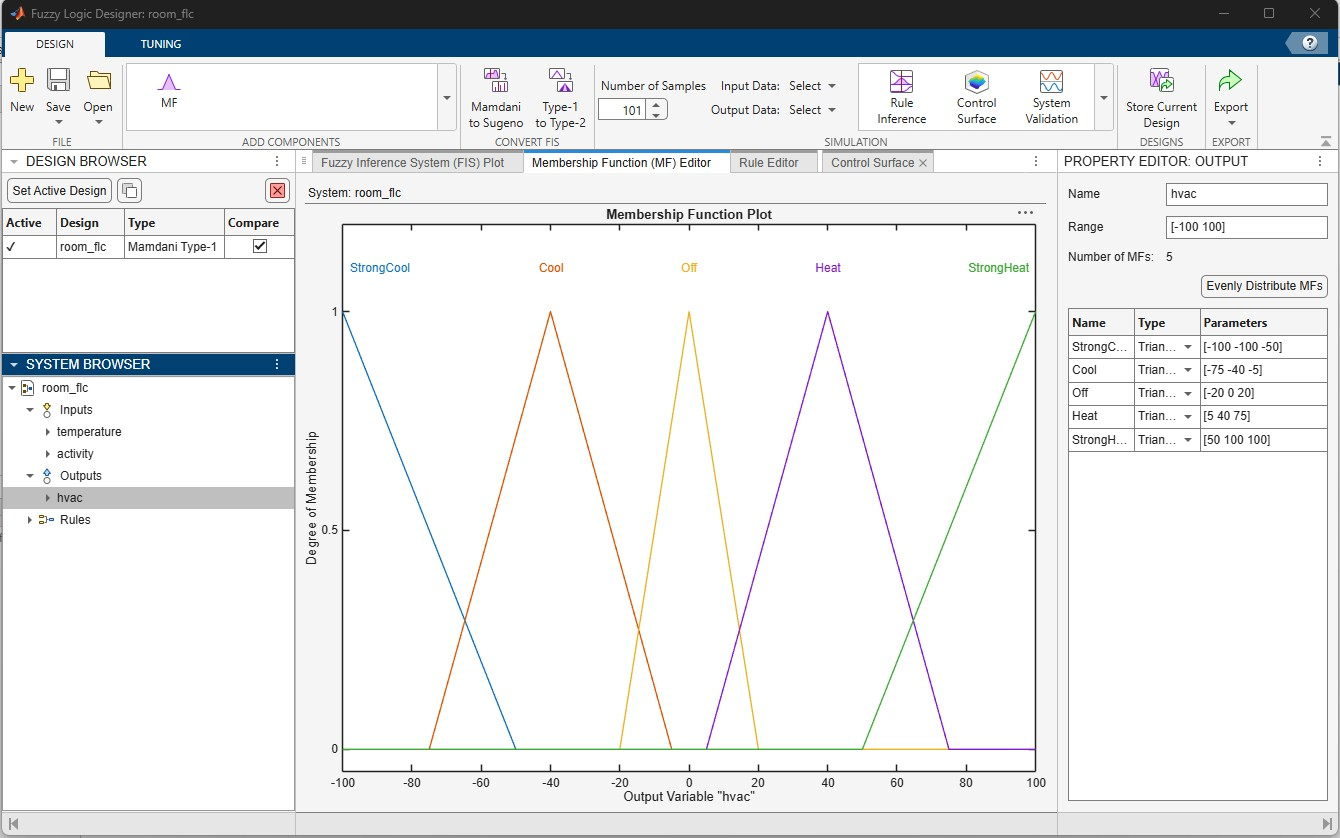
\includegraphics[width=\textwidth]{../realss/gui_05_mf_hvac.jpg}\\[1pt]
    {\small (c) hvac}
  \end{minipage}
  \caption{Membership-function editor in the Fuzzy Logic Designer for the two inputs and the output, each
  with its membership-function parameter table on the right.}
  \label{fig:gui_mf}
\end{figure}

\begin{figure}[h]
  \centering
  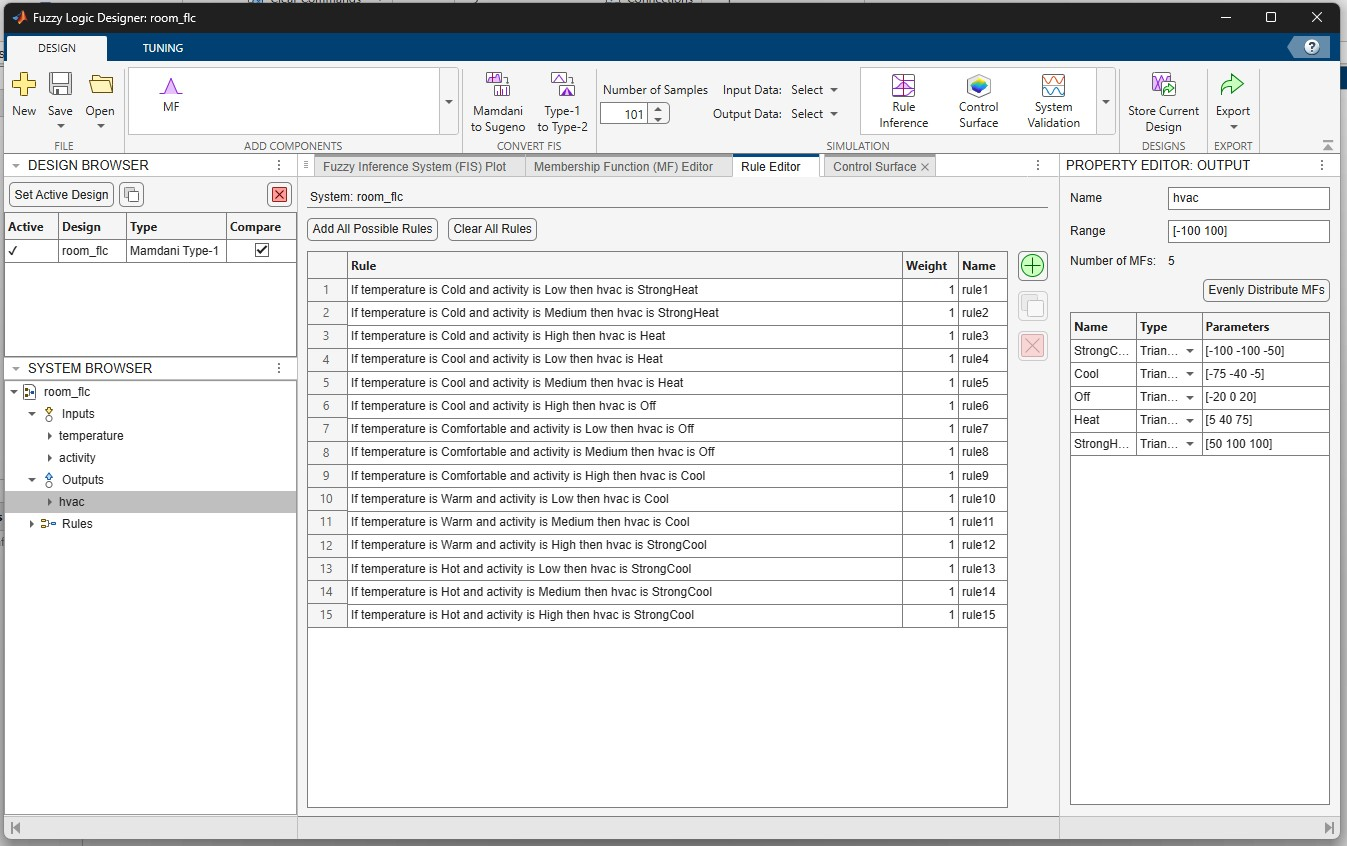
\includegraphics[width=0.92\textwidth]{../realss/gui_06_rules.jpg}
  \caption{Rule editor: the complete 15-rule base shown in natural language inside the designer.}
  \label{fig:gui_rules}
\end{figure}

\begin{figure}[h]
  \centering
  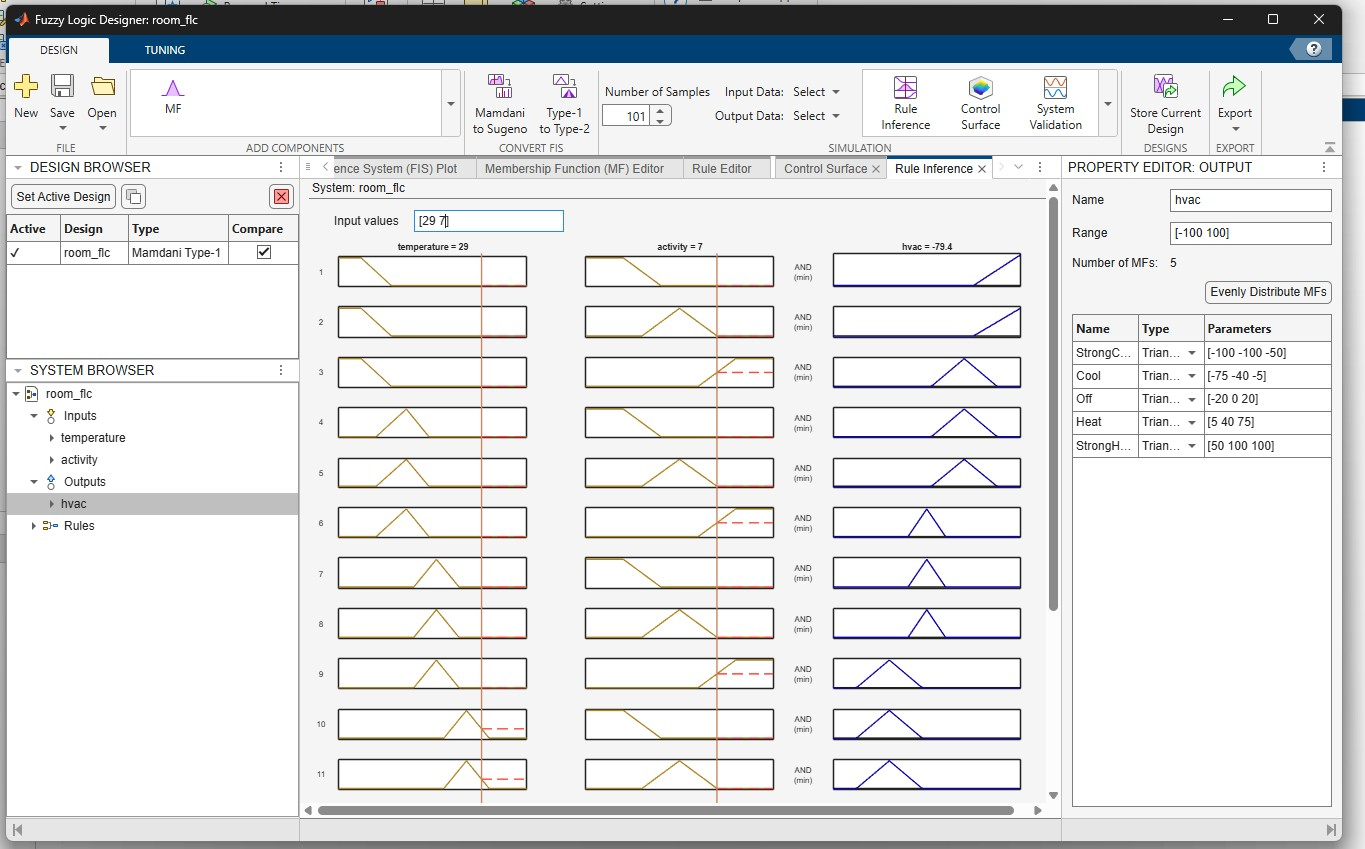
\includegraphics[width=0.95\textwidth]{../realss/gui_07_inference.jpg}
  \caption{Rule Inference view at temperature 29 and activity 7. Only the rules whose antecedents overlap
  the inputs fire, and the aggregated, defuzzified command is \(-79.4\) (strong cooling), matching the
  programmatic result in Figure~\ref{fig:p1rule}.}
  \label{fig:gui_infer}
\end{figure}

\begin{figure}[h]
  \centering
  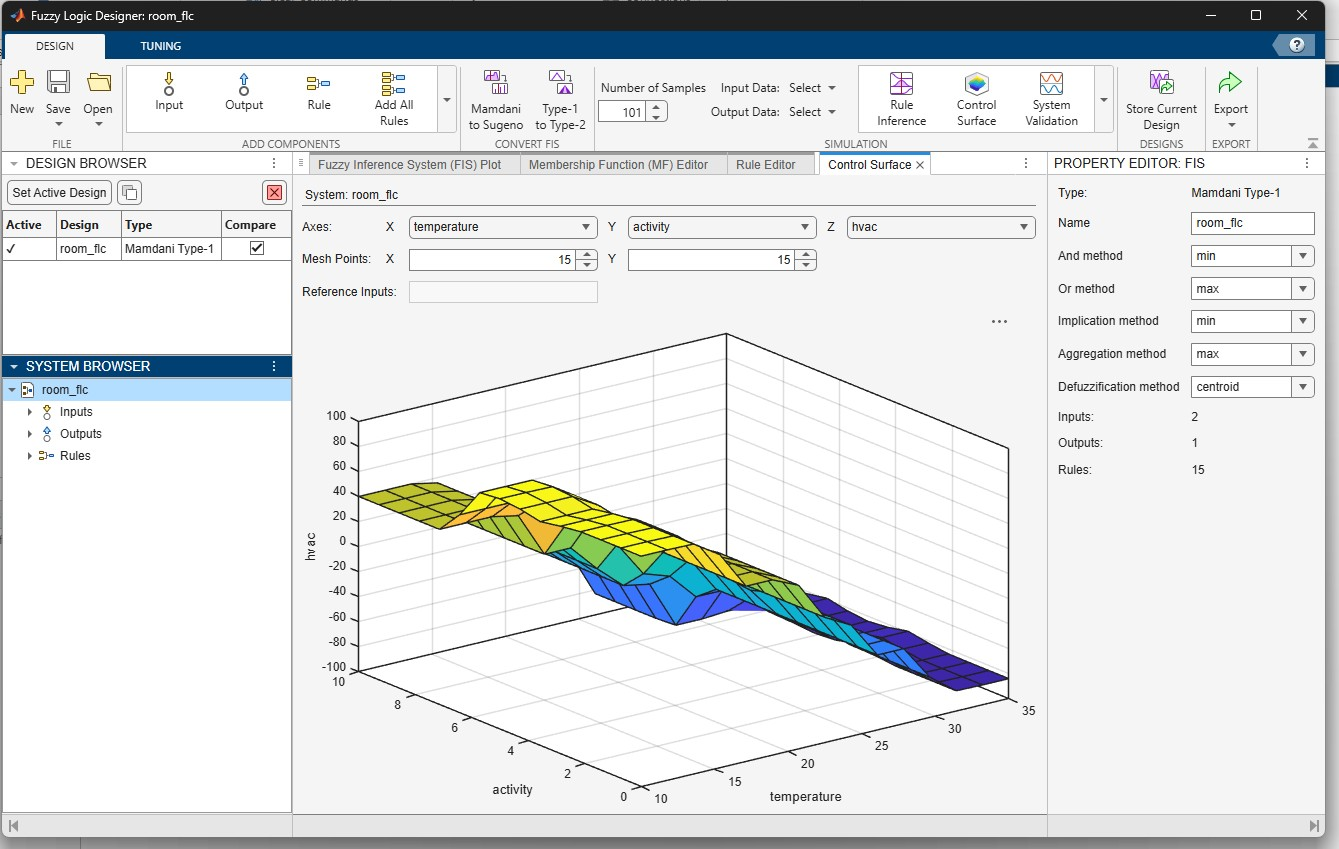
\includegraphics[width=0.92\textwidth]{../realss/gui_01_surface.jpg}
  \caption{Interactive control surface in the Fuzzy Logic Designer, the GUI counterpart of
  Figure~\ref{fig:p1surf}.}
  \label{fig:gui_surface}
\end{figure}

\clearpage
%======================================================================
\section{Part 2: Optimising the FLC with a Genetic Algorithm}
%======================================================================

\subsection{Target dataset}
The module does not provide a labelled dataset, so we generate one from a smooth, physically motivated
target response and state this clearly. The desired command is a saturating proportional law around a
neutral temperature that decreases with activity:
\begin{equation}
  y^{\star}(\text{temp},\text{act}) = 100\,\tanh\!\big(-0.14\,(\text{temp} - (24 - 0.6\,\text{act}))\big),
\end{equation}
clamped to $[-100,100]$. We sample this on a grid of temperature $\{10,11,\dots,35\}$ and activity
$\{0,1,\dots,10\}$, giving 286 examples, and add mild Gaussian noise (standard deviation 2) to mimic
sensor variation (see \texttt{make\_dataset.m}). The fixed neutral point of \SI{24}{\celsius} at rest,
falling by \SI{0.6}{\celsius} per unit of activity, encodes the same comfort knowledge as the rule base
but as a continuous reference the GA can fit against.

\subsection{Problem encoding and chromosome length}
The chromosome is a real-valued vector of the membership-function breakpoints of the input and output
variables. To keep every candidate a valid fuzzy partition, the two outermost anchors of the first and
last set on each variable are pinned to the ends of that variable's range, and all remaining breakpoints
are tuned. On decoding, each membership function's breakpoints are clamped to the variable range and
sorted into non-decreasing order, which repairs any ordering that crossover or mutation may break
(see \texttt{flc\_template.m} and \texttt{flc\_decode.m}). Counting the free breakpoints gives a
\textbf{chromosome length of $L = 31$} genes: 13 for temperature, 7 for activity and 11 for the HVAC
output.

\subsection{Genetic operators}
The genetic algorithm is real-coded and hand-implemented (\texttt{ga\_optimise\_flc.m}):
\begin{itemize}
  \item \textbf{Selection:} tournament selection with tournament size 3.
  \item \textbf{Crossover:} BLX-$\alpha$ (blend) crossover with $\alpha = 0.5$ and crossover rate 0.9.
  \item \textbf{Mutation:} per-gene Gaussian mutation at rate 0.15 with standard deviation equal to
        10 percent of each gene's range.
  \item \textbf{Repair:} clamp to range and sort the breakpoints of each membership function.
  \item \textbf{Elitism:} the best 2 individuals are copied unchanged into the next generation.
  \item \textbf{Population and generations:} 50 individuals for 80 generations. One individual is seeded
        with the hand-designed controller and the rest are random or perturbed, which preserves expert
        knowledge while still exploring the search space.
\end{itemize}

\subsection{Fitness function}
Fitness is the mean squared error between the controller output and the target over the dataset, which the
GA minimises:
\begin{equation}
  \mathrm{MSE} = \frac{1}{n}\sum_{i=1}^{n}\big(\widehat{y}(x_i) - y^{\star}_i\big)^2,
  \qquad \widehat{y}(x_i) = \texttt{evalfis}(\text{FIS}, x_i).
\end{equation}
Candidates that leave a coverage gap (so that no rule fires for some input) are penalised automatically
because the controller then returns its mid-range value and the error grows.

\subsection{Results}
The GA reduced the error substantially, as summarised in Table~\ref{tab:ga} and
Figure~\ref{fig:p2conv}. The mean squared error fell from 300.9 for the hand-designed controller to 57.2,
a reduction of 81 percent (root mean squared error from 17.3 to 7.6 on the $[-100,100]$ command scale).
Notably, the hand-coded GA also beat MATLAB's built-in \texttt{ga} solver (which reached 136.7 under the
same evaluation budget), because the blend crossover and the knowledge-seeded population suit this
bounded, ordered encoding well.

\begin{table}[h]
  \centering
  \caption{Part 2 results. MSE and RMSE of the fuzzy controller against the target dataset before and
  after optimisation, with the Global Optimization Toolbox \texttt{ga} solver as an independent check.}
  \label{tab:ga}
  \begin{tabular}{lccc}
    \toprule
    & \textbf{MSE} & \textbf{RMSE} & \textbf{Notes} \\
    \midrule
    Hand-designed FLC (baseline) & 300.85 & 17.35 & expert rules and sets \\
    Hand-coded GA                & \textbf{57.15} & \textbf{7.56} & 81\% lower MSE \\
    Built-in \texttt{ga} (check) & 136.69 & 11.69 & same budget \\
    \bottomrule
  \end{tabular}
\end{table}

\begin{figure}[h]
  \centering
  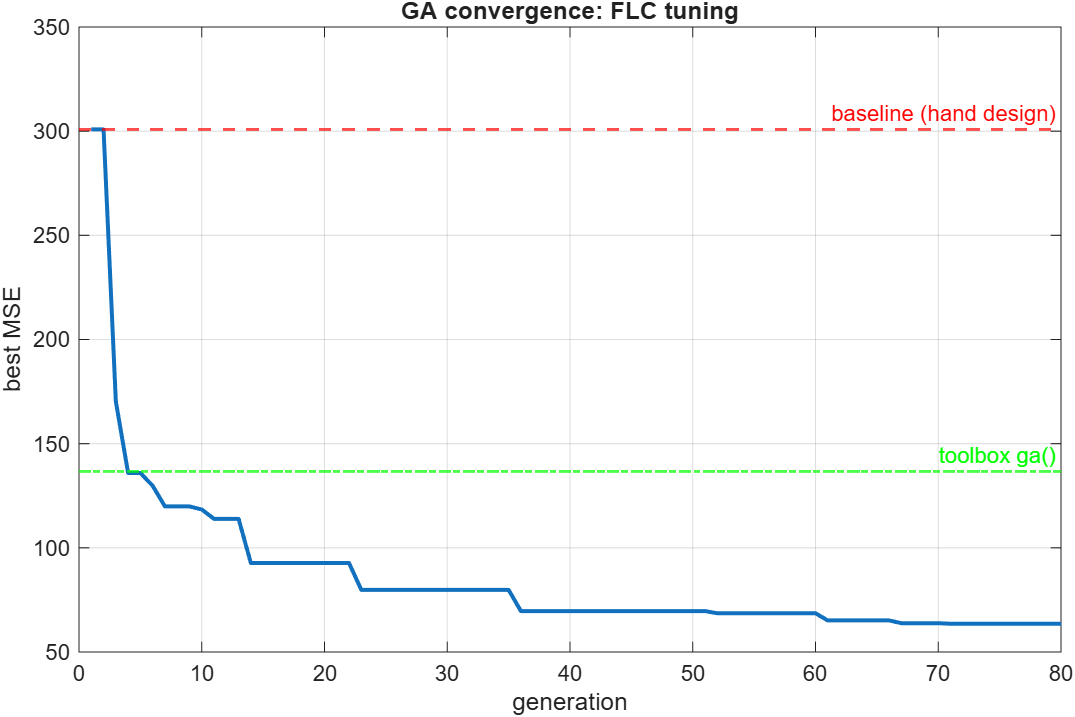
\includegraphics[width=0.7\textwidth]{p2_convergence.png}
  \caption{GA convergence. The best MSE drops below the hand-designed baseline within a few generations
  and below the built-in \texttt{ga} result, settling near 57 after 80 generations.}
  \label{fig:p2conv}
\end{figure}

The optimiser reshaped the membership functions (Figure~\ref{fig:p2mf}) and produced a smoother
input-output map that follows the target more closely (Figures~\ref{fig:p2surf}
and~\ref{fig:p2pred}). The GA widens and repositions the temperature and HVAC sets so that the
interpolation matches the saturating target law more faithfully than the evenly spaced hand design.

\begin{figure}[h]
  \centering
  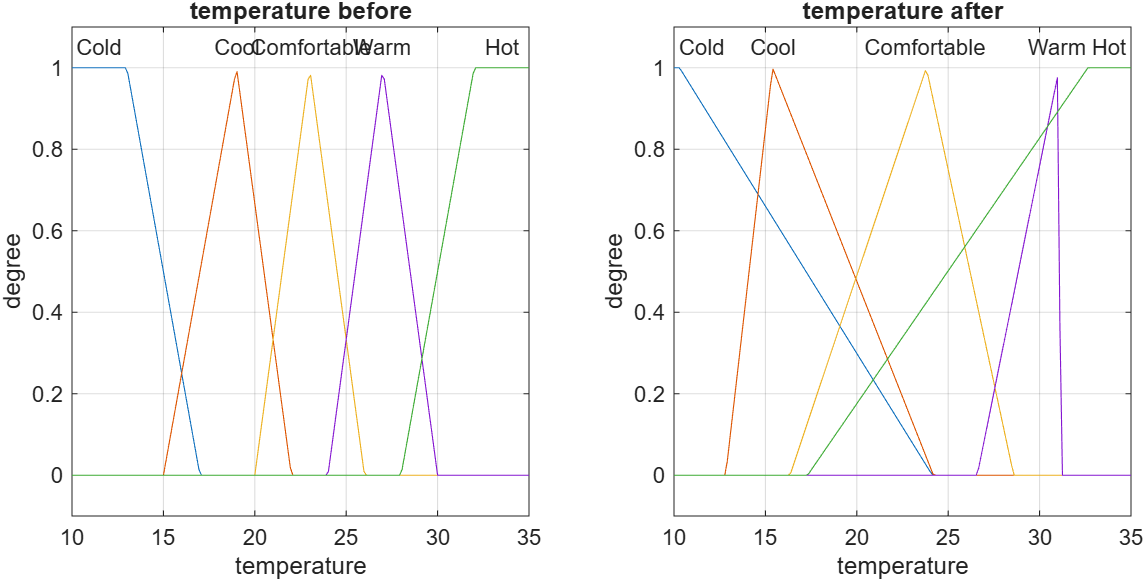
\includegraphics[width=0.95\textwidth]{p2_mf_temperature_ba.png}
  \caption{Temperature membership functions before (left) and after (right) GA optimisation. The GA moves
  and reshapes the sets to better match the target response.}
  \label{fig:p2mf}
\end{figure}

\begin{figure}[h]
  \centering
  \begin{minipage}{0.49\textwidth}
    \centering
    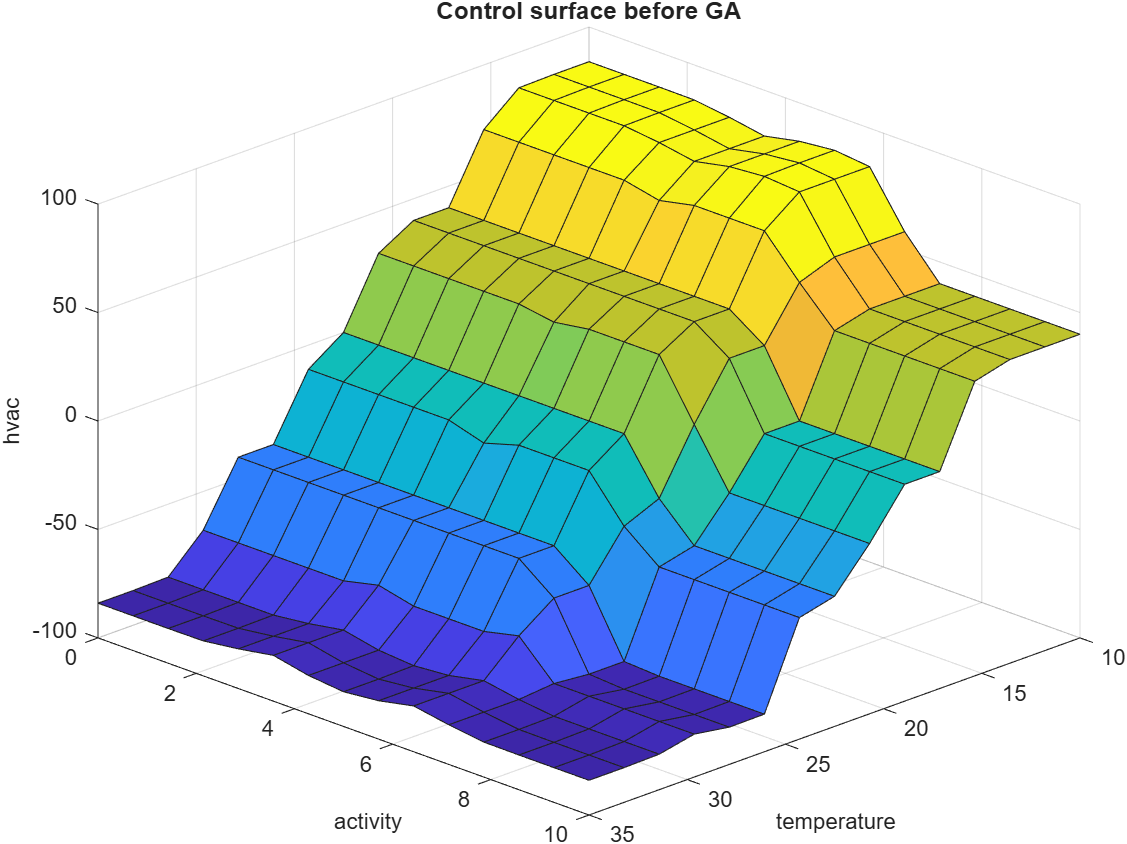
\includegraphics[width=\textwidth]{p2_surface_before.png}\\
    {\small (a) Before GA}
  \end{minipage}
  \hfill
  \begin{minipage}{0.49\textwidth}
    \centering
    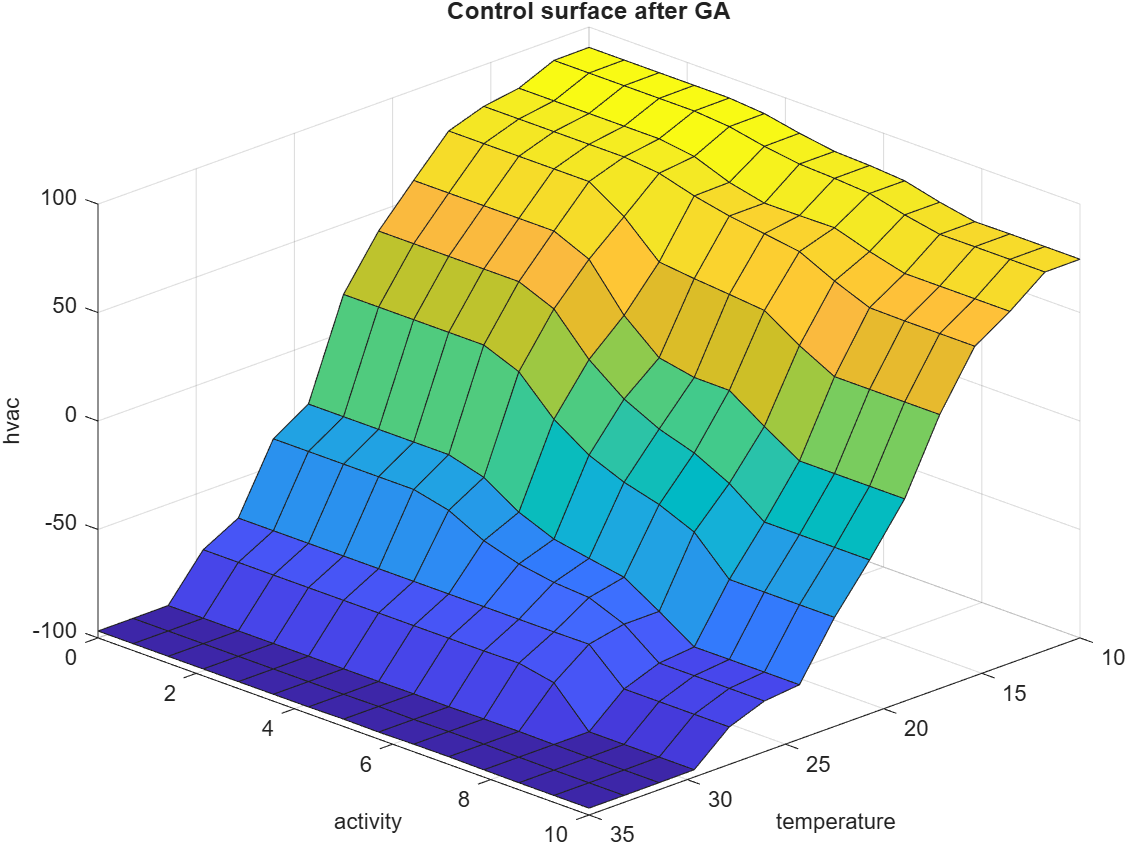
\includegraphics[width=\textwidth]{p2_surface_after.png}\\
    {\small (b) After GA}
  \end{minipage}
  \caption{Control surface before and after optimisation. The optimised surface is smoother and tracks the
  target comfort law more closely.}
  \label{fig:p2surf}
\end{figure}

\begin{figure}[h]
  \centering
  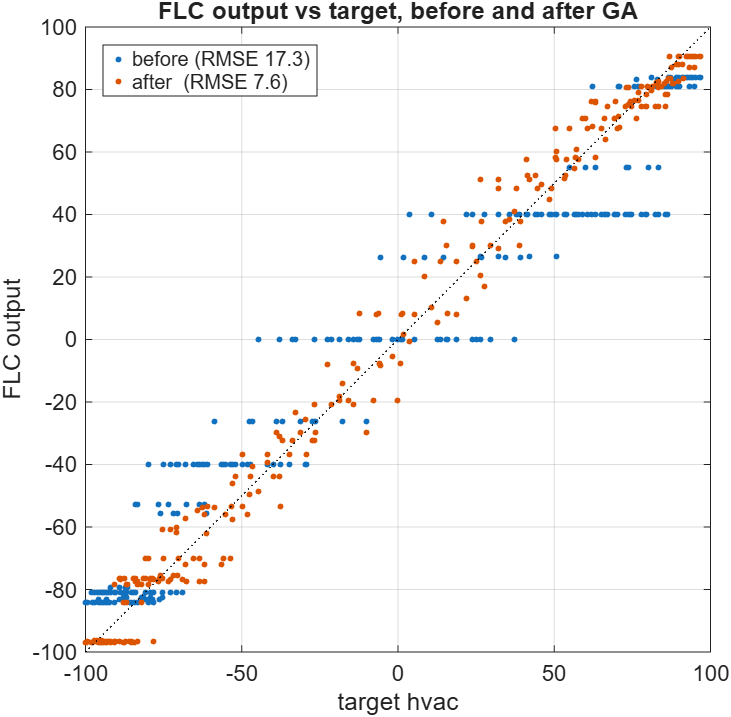
\includegraphics[width=0.66\textwidth]{p2_pred_vs_target.png}
  \caption{Controller output against the target for all 286 examples. After optimisation the points lie
  much closer to the diagonal, confirming the lower error.}
  \label{fig:p2pred}
\end{figure}

\subsection{How the solution would change for a Sugeno model}
If the controller were a Sugeno (Takagi-Sugeno) system, each rule consequent would be a constant or a
linear function of the inputs rather than an output fuzzy set. The input encoding would be unchanged (the
GA would still tune the input membership-function breakpoints), but the output part of the chromosome
would no longer encode the breakpoints of the five output sets. Instead it would encode the consequent
coefficients: one constant per rule for a zero-order Sugeno system, or, for a first-order system,
$(\text{slope}_\text{temp}, \text{slope}_\text{act}, \text{offset})$ per rule. With 15 rules a zero-order
Sugeno output would contribute 15 genes (constants) and a first-order output 45 genes, replacing the 11
output-breakpoint genes used here. Two practical effects follow: the ordering and clamping repair would no
longer be needed for the output (consequent coefficients are unconstrained), and fitness evaluation would
be faster because Sugeno defuzzification is a weighted average rather than a centroid over an aggregated
fuzzy set. The reverse change, from Sugeno to Mamdani, would replace the consequent coefficient genes with
output membership-function breakpoint genes and reinstate the ordering repair.

\clearpage
%======================================================================
\section{Part 3: Comparison of Optimisers on CEC'2005 Functions}
%======================================================================

\subsection{Benchmark functions}
We use two functions from the CEC'2005 special-session suite, one unimodal and one multimodal, so that the
comparison covers both easy and hard landscapes (Figure~\ref{fig:p3land}):
\begin{itemize}
  \item \textbf{F1, Shifted Sphere} (unimodal):
        $f_1(\mathbf{x}) = \sum_{i=1}^{D}(x_i - o_i)^2 + f_\text{bias}$, with $f_\text{bias} = -450$ and
        search range $[-100,100]^D$. The global minimum is $-450$ at $\mathbf{x}=\mathbf{o}$.
  \item \textbf{F9, Shifted Rastrigin} (multimodal):
        $f_9(\mathbf{x}) = \sum_{i=1}^{D}\big(z_i^2 - 10\cos(2\pi z_i) + 10\big) + f_\text{bias}$,
        with $\mathbf{z} = \mathbf{x}-\mathbf{o}$, $f_\text{bias} = -330$ and range $[-5,5]^D$. The global
        minimum is $-330$. Rastrigin has a very large number of regularly spaced local minima, which makes
        it a standard test of an optimiser's ability to escape local optima.
\end{itemize}
Each function is shifted by a fixed vector $\mathbf{o}$ so the optimum is not at the origin. The shift is
generated once with a fixed seed and stored (see \texttt{cec\_setup.m} and \texttt{cec\_problem.m}), so
every run is reproducible and the optimum lies in the interior of the domain. We report the error
$f(\mathbf{x}) - f^{\star}$, the distance of the best found value from the known optimum.

\begin{figure}[h]
  \centering
  \begin{minipage}{0.49\textwidth}
    \centering
    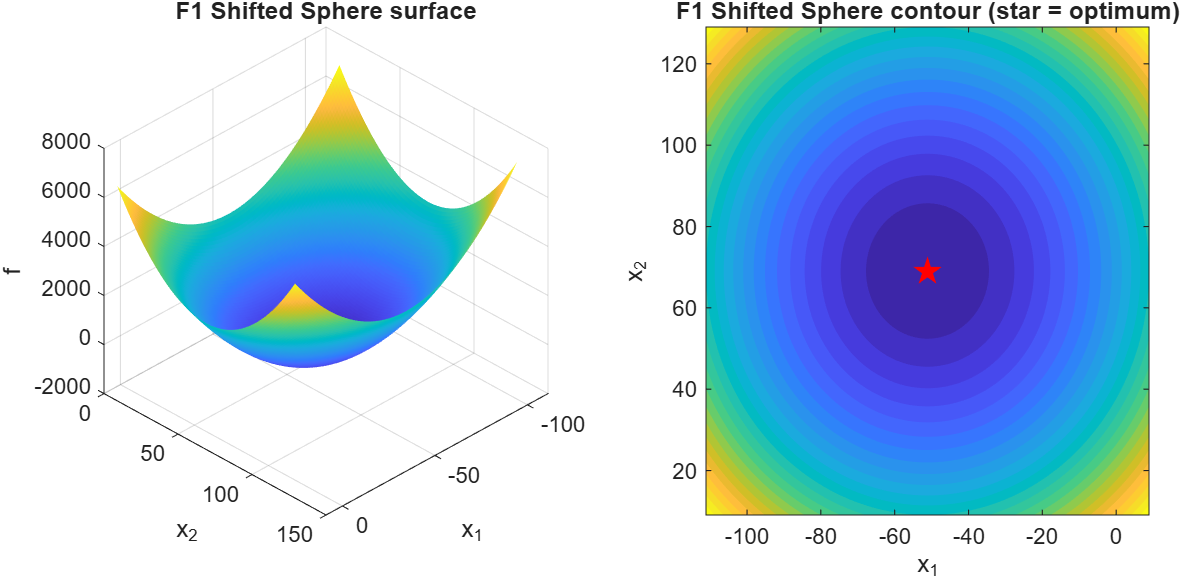
\includegraphics[width=\textwidth]{p3_landscape_F1.png}\\
    {\small (a) F1 Shifted Sphere}
  \end{minipage}
  \hfill
  \begin{minipage}{0.49\textwidth}
    \centering
    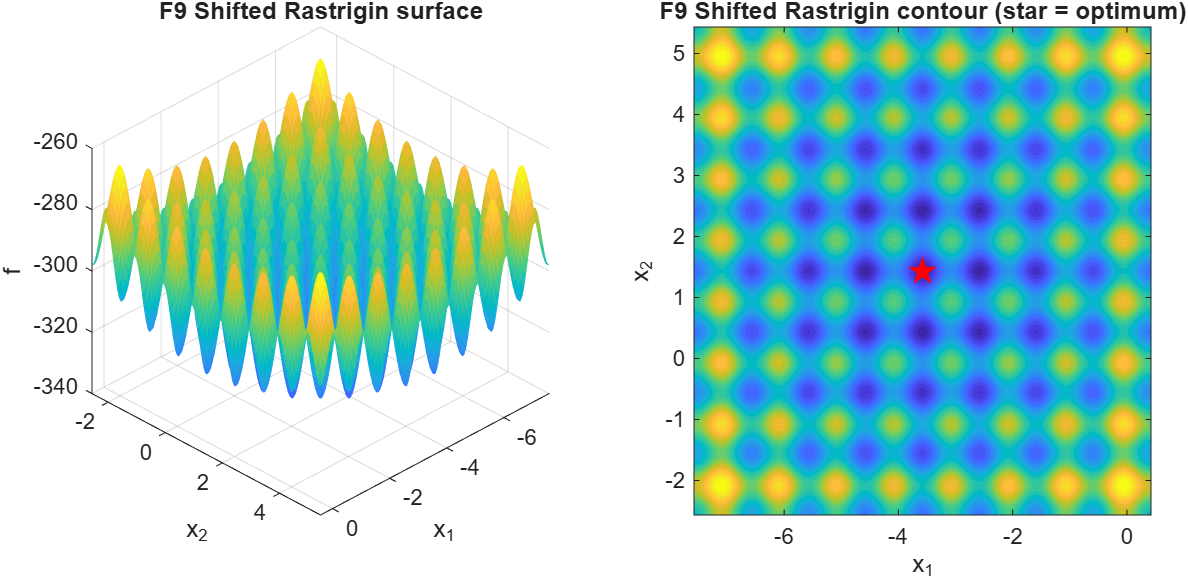
\includegraphics[width=\textwidth]{p3_landscape_F9.png}\\
    {\small (b) F9 Shifted Rastrigin}
  \end{minipage}
  \caption{Surface and contour of the two benchmark functions at $D=2$. The sphere is a single smooth
  bowl; Rastrigin is covered in regularly spaced local minima around the global optimum (red star).}
  \label{fig:p3land}
\end{figure}

\subsection{Optimisers and parameters}
Three optimisers were implemented from scratch (\texttt{opt\_ga.m}, \texttt{opt\_pso.m},
\texttt{opt\_sa.m}):
\begin{itemize}
  \item \textbf{Genetic algorithm (GA):} real-coded, population 50, tournament selection (size 3),
        BLX-0.5 crossover, Gaussian mutation (rate 0.10), elitism of the best 2.
  \item \textbf{Particle swarm optimisation (PSO):} swarm size 40, inertia $w = 0.729$, cognitive and
        social coefficients $c_1 = c_2 = 1.49445$ (the standard Clerc constriction values), velocity
        clamped to 20 percent of the range.
  \item \textbf{Simulated annealing (SA):} geometric cooling from an initial temperature estimated from
        the spread of a random sample, Gaussian proposals whose step shrinks as the temperature falls, and
        Metropolis acceptance.
\end{itemize}

\subsection{Experimental protocol}
Following the CEC'2005 guidelines, each optimiser is run with a budget of $\text{maxFES} = 10000 \times D$
function evaluations. Every configuration (function $\times$ dimension $\times$ optimiser) is repeated for
\textbf{15 independent runs} at $D = 2$ and $D = 10$. We report the mean, standard deviation, best and
worst final error over the 15 runs, and the best-so-far error averaged over the runs as a convergence
graph.

\subsection{Results}
Table~\ref{tab:p3} gives the statistics and Figure~\ref{fig:p3conv} shows the averaged convergence. On the
unimodal Sphere all three optimisers solve the problem at $D=2$, and GA and PSO reach the optimum to high
precision at $D=10$; SA is less precise because its step size limits the final refinement, and PSO shows
occasional stagnation at $D=10$ (a high worst-case run that inflates its mean and standard deviation). On
the multimodal Rastrigin function the picture changes: at $D=10$ the GA is clearly the most robust, with a
mean error of about 0.02, while PSO and SA become trapped in local minima with mean errors of about 11 and
22 respectively. The convergence graph for Rastrigin at $D=10$ shows this clearly: the GA keeps descending
throughout the budget while PSO and SA flatten early.

\begin{table}[h]
  \centering
  \caption{CEC'2005 comparison: error $f - f^{\star}$ over 15 runs, budget $10000\times D$ evaluations.
  Best mean per configuration in bold.}
  \label{tab:p3}
  \footnotesize
  \begin{tabular}{ll l rrrr}
    \toprule
    \textbf{Function} & \textbf{D} & \textbf{Opt} & \textbf{Mean} & \textbf{Std} & \textbf{Best} & \textbf{Worst} \\
    \midrule
    F1 Sphere    & 2  & GA  & \textbf{0.00e+00} & 0.00e+00 & 0.00e+00 & 0.00e+00 \\
    F1 Sphere    & 2  & PSO & \textbf{0.00e+00} & 0.00e+00 & 0.00e+00 & 0.00e+00 \\
    F1 Sphere    & 2  & SA  & 1.61e$-$01 & 3.17e$-$01 & 6.21e$-$03 & 1.27e+00 \\
    \midrule
    F1 Sphere    & 10 & GA  & 1.10e$-$02 & 5.65e$-$03 & 2.21e$-$03 & 2.12e$-$02 \\
    F1 Sphere    & 10 & PSO & 6.38e+01 & 2.47e+02 & \textbf{0.00e+00} & 9.57e+02 \\
    F1 Sphere    & 10 & SA  & 8.89e+00 & 6.48e+00 & 2.94e+00 & 2.95e+01 \\
    \midrule
    F9 Rastrigin & 2  & GA  & 9.35e$-$12 & 3.62e$-$11 & 0.00e+00 & 1.40e$-$10 \\
    F9 Rastrigin & 2  & PSO & \textbf{0.00e+00} & 0.00e+00 & 0.00e+00 & 0.00e+00 \\
    F9 Rastrigin & 2  & SA  & 4.19e$-$01 & 4.60e$-$01 & 5.05e$-$07 & 1.06e+00 \\
    \midrule
    F9 Rastrigin & 10 & GA  & \textbf{1.80e$-$02} & 1.14e$-$02 & 4.97e$-$03 & 4.17e$-$02 \\
    F9 Rastrigin & 10 & PSO & 1.14e+01 & 6.52e+00 & 2.98e+00 & 2.88e+01 \\
    F9 Rastrigin & 10 & SA  & 2.16e+01 & 9.18e+00 & 4.98e+00 & 3.84e+01 \\
    \bottomrule
  \end{tabular}
\end{table}

\begin{figure}[h]
  \centering
  \begin{minipage}{0.49\textwidth}
    \centering
    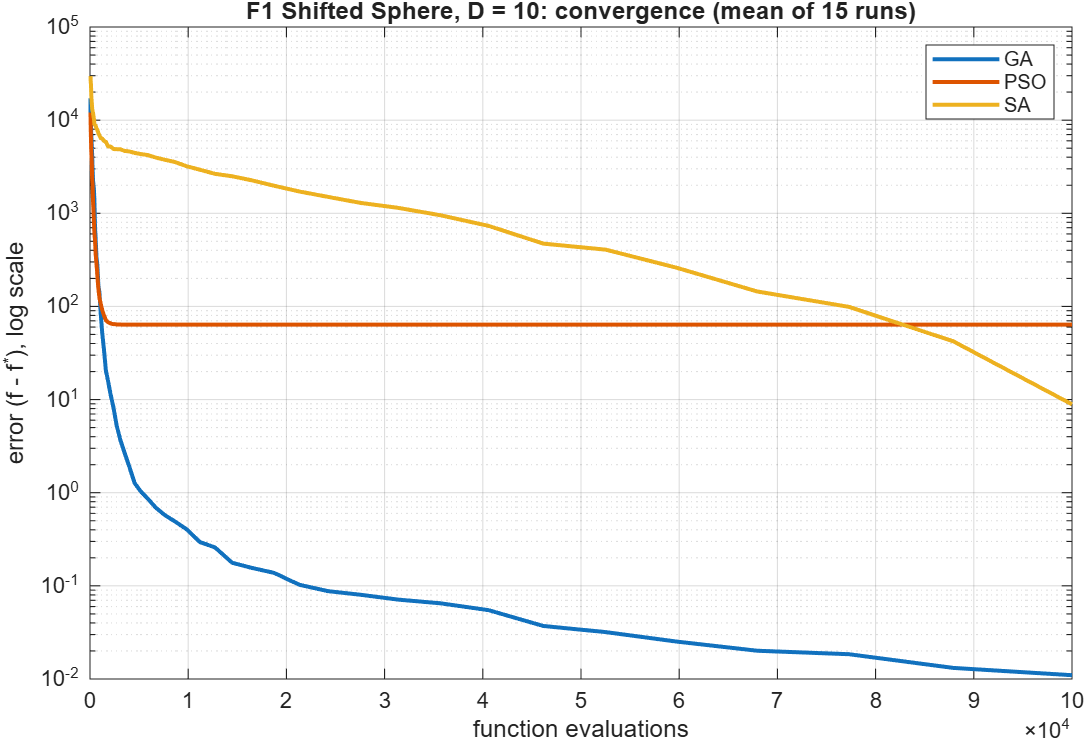
\includegraphics[width=\textwidth]{p3_conv_F1_D10.png}\\
    {\small (a) F1 Sphere, $D=10$}
  \end{minipage}
  \hfill
  \begin{minipage}{0.49\textwidth}
    \centering
    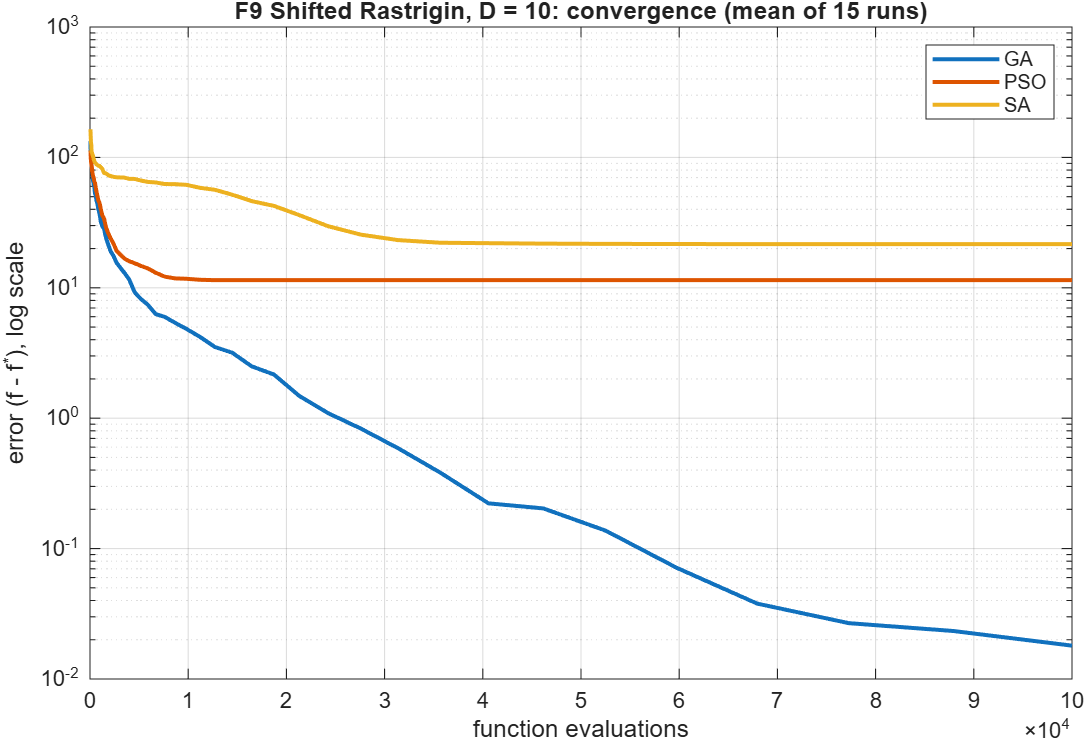
\includegraphics[width=\textwidth]{p3_conv_F9_D10.png}\\
    {\small (b) F9 Rastrigin, $D=10$}
  \end{minipage}
  \caption{Averaged best-so-far error (log scale) against function evaluations at $D=10$. On the sphere GA
  and PSO converge fastest; on Rastrigin the GA keeps improving while PSO and SA stall in local minima.}
  \label{fig:p3conv}
\end{figure}

\subsection{Cross-check against the Global Optimization Toolbox}
To validate the hand-coded optimisers we ran the toolbox solvers \texttt{ga}, \texttt{particleswarm} and
\texttt{simulannealbnd} on the same problems and budget for 15 runs (\texttt{compare\_cec\_toolbox.m},
Table~\ref{tab:p3tb}). The pattern matches our implementations: \texttt{particleswarm} is excellent on the
smooth sphere and \texttt{ga} is the most robust on Rastrigin at $D=10$. The toolbox \texttt{particleswarm}
avoids the occasional stagnation seen in our simpler PSO because it includes adaptive neighbourhood and
restart mechanisms, while our hand-coded GA is competitive with, and on Rastrigin slightly different from,
the toolbox \texttt{ga}. The agreement gives confidence that the comparison reflects the algorithms rather
than implementation errors.

\begin{table}[h]
  \centering
  \caption{Global Optimization Toolbox cross-check: error $f - f^{\star}$ over 15 runs, same budget.}
  \label{tab:p3tb}
  \footnotesize
  \begin{tabular}{ll l rrrr}
    \toprule
    \textbf{Function} & \textbf{D} & \textbf{Solver} & \textbf{Mean} & \textbf{Std} & \textbf{Best} & \textbf{Worst} \\
    \midrule
    F1 Sphere    & 2  & \texttt{ga}             & 6.42e$-$10 & 9.68e$-$10 & 1.76e$-$12 & 3.12e$-$09 \\
    F1 Sphere    & 2  & \texttt{particleswarm}  & 1.30e$-$08 & 1.79e$-$08 & 5.91e$-$12 & 5.18e$-$08 \\
    F1 Sphere    & 2  & \texttt{simulannealbnd} & 1.69e$-$05 & 6.08e$-$05 & 3.29e$-$10 & 2.36e$-$04 \\
    \midrule
    F1 Sphere    & 10 & \texttt{ga}             & 1.01e$-$03 & 1.07e$-$03 & 1.50e$-$05 & 4.41e$-$03 \\
    F1 Sphere    & 10 & \texttt{particleswarm}  & 2.22e$-$05 & 2.30e$-$05 & 3.10e$-$06 & 8.77e$-$05 \\
    F1 Sphere    & 10 & \texttt{simulannealbnd} & 4.61e$-$01 & 2.59e$-$01 & 1.61e$-$01 & 8.86e$-$01 \\
    \midrule
    F9 Rastrigin & 2  & \texttt{ga}             & 3.32e$-$01 & 6.14e$-$01 & 2.30e$-$10 & 1.99e+00 \\
    F9 Rastrigin & 2  & \texttt{particleswarm}  & 1.28e$-$07 & 4.49e$-$07 & 0.00e+00 & 1.75e$-$06 \\
    F9 Rastrigin & 2  & \texttt{simulannealbnd} & 4.19e$-$01 & 4.93e$-$01 & 4.54e$-$09 & 9.95e$-$01 \\
    \midrule
    F9 Rastrigin & 10 & \texttt{ga}             & 2.52e+00 & 4.19e+00 & 1.65e$-$04 & 1.49e+01 \\
    F9 Rastrigin & 10 & \texttt{particleswarm}  & 1.17e+01 & 6.83e+00 & 4.97e+00 & 3.10e+01 \\
    F9 Rastrigin & 10 & \texttt{simulannealbnd} & 1.80e+01 & 6.15e+00 & 1.10e+01 & 2.99e+01 \\
    \bottomrule
  \end{tabular}
\end{table}

\subsection{Discussion and comparison with the literature}
The results agree with the established understanding of these algorithms. The Sphere function is convex and
separable, so a swarm with momentum converges to it very quickly, which is why PSO and the GA reach the
optimum on it. Rastrigin is the harder test: its dense local minima cause local search and momentum-based
methods to stall, and the published CEC'2005 results report that simple optimisers leave a clear residual
error on shifted Rastrigin at $D=10$, exactly as our PSO and SA do. The GA performs best here because its
population maintains diversity and its crossover recombines partial solutions across the many basins, which
is the recognised strength of population-based recombination on rugged multimodal landscapes. The increase
in error from $D=2$ to $D=10$ for every optimiser also reflects the curse of dimensionality noted
throughout the benchmark literature.

%======================================================================
\section{Conclusion}
%======================================================================
We designed, implemented and analysed a Mamdani fuzzy logic controller for thermal comfort in an assistive
care room, optimised its membership functions with a hand-coded genetic algorithm, and compared three
evolutionary optimisers on two CEC'2005 benchmark functions. The controller behaves correctly across rule
activation, the control surface and a full day-long scenario. The genetic algorithm cut the fitting error
by 81 percent and outperformed the built-in solver on the same problem. On the benchmark comparison the
genetic algorithm was the most robust optimiser on the multimodal function, particle swarm was strongest on
the smooth function, and simulated annealing was weakest at high dimension; the hand-coded optimisers
agreed with the Global Optimization Toolbox solvers. Future work could add a third input such as humidity,
optimise the rule weights as well as the membership functions, and extend the benchmark study to $D=100$
and to rotated CEC'2005 functions.

%======================================================================
\section*{Author Contributions}
%======================================================================
Rahul Karn (250163) led the fuzzy logic controller design and implementation (Part 1) and the genetic
algorithm optimisation (Part 2), including the dataset, encoding and fitness function. Rashant Nayaju
(250117) led the CEC'2005 optimiser comparison (Part 3), including the benchmark functions, the
particle swarm and simulated annealing implementations, and the experimental protocol. Both authors
contributed to the genetic algorithm, the analysis of results and the writing of this report.

%======================================================================
\begin{thebibliography}{9}
%======================================================================
\bibitem{zadeh} L. A. Zadeh, ``Fuzzy sets,'' \emph{Information and Control}, vol. 8, no. 3, pp. 338--353, 1965.
\bibitem{mamdani} E. H. Mamdani and S. Assilian, ``An experiment in linguistic synthesis with a fuzzy logic controller,'' \emph{International Journal of Man-Machine Studies}, vol. 7, no. 1, pp. 1--13, 1975.
\bibitem{sugeno} T. Takagi and M. Sugeno, ``Fuzzy identification of systems and its applications to modeling and control,'' \emph{IEEE Transactions on Systems, Man, and Cybernetics}, vol. SMC-15, no. 1, pp. 116--132, 1985.
\bibitem{holland} J. H. Holland, \emph{Adaptation in Natural and Artificial Systems}. Ann Arbor: University of Michigan Press, 1975.
\bibitem{goldberg} D. E. Goldberg, \emph{Genetic Algorithms in Search, Optimization, and Machine Learning}. Addison-Wesley, 1989.
\bibitem{pso} J. Kennedy and R. Eberhart, ``Particle swarm optimization,'' in \emph{Proc. IEEE International Conference on Neural Networks}, 1995, pp. 1942--1948.
\bibitem{sa} S. Kirkpatrick, C. D. Gelatt, and M. P. Vecchi, ``Optimization by simulated annealing,'' \emph{Science}, vol. 220, no. 4598, pp. 671--680, 1983.
\bibitem{cec2005} P. N. Suganthan, N. Hansen, J. J. Liang, K. Deb, Y.-P. Chen, A. Auger, and S. Tiwari, ``Problem definitions and evaluation criteria for the CEC 2005 special session on real-parameter optimization,'' Nanyang Technological University, Tech. Rep., 2005.
\bibitem{matlab} The MathWorks, \emph{Fuzzy Logic Toolbox and Global Optimization Toolbox User's Guides}, MATLAB R2026a, 2026.
\end{thebibliography}

\clearpage
%======================================================================
\appendix
\section{Code Availability}
%======================================================================
All MATLAB source for this task (the fuzzy controller, the genetic algorithm, the CEC'2005 functions and
the optimisers, together with the figures and result tables) is available in the project repository:

\begin{center}
\url{https://github.com/rahulkarn250163/aml} \quad (folder \texttt{task2/})
\end{center}

The complete pipeline can be reproduced from the \texttt{task2/} folder in MATLAB by running
\texttt{run\_all}. As required for Part~3, the MATLAB code for the two benchmark functions used in the
comparison is listed below; the remaining scripts (the FLC, the genetic algorithm, the optimisers and the
comparison harness) are in the repository.

\subsection{CEC'2005 benchmark functions (Part 3)}
\lstinputlisting[caption={cec2005/cec\_problem.m, which defines F1 Shifted Sphere and F9 Shifted Rastrigin}]{../cec2005/cec_problem.m}
\lstinputlisting[caption={cec2005/cec\_setup.m, which generates and stores the fixed shift vectors}]{../cec2005/cec_setup.m}

\end{document}
